\documentclass{article} % Especially this!

%%%%%%%%%%%%%%%%%%%%%%%%%%%%%%%%%%%%%%%%%%%%%%%%%%%%%%%%

\usepackage[english]{babel}
\usepackage[utf8]{inputenc}
\usepackage[a4paper, total={6in, 8.5in}]{geometry}
\usepackage{amsmath}
\usepackage{amsthm}
\usepackage{amsfonts}
\usepackage{amssymb}
\usepackage[usenames,dvipsnames]{xcolor}
\usepackage{graphicx}
%\usepackage[siunitx]{circuitikz}
\usepackage{tikz}
\usepackage[ruled,vlined]{algorithm2e}
\usepackage[colorinlistoftodos, color=orange!50]{todonotes}
\usepackage{hyperref}
\usepackage[numbers, square]{natbib}
\usepackage{fancybox}
\usepackage{epsfig}
\usepackage{soul}
\usepackage{listings}
\usepackage[framemethod=tikz]{mdframed}
\usepackage[shortlabels]{enumitem}
\usepackage[version=4]{mhchem}
\usepackage{multicol}
\usepackage{pgfplots}
\usepackage{version}
\pgfplotsset{compat=1.14}
\usepackage{graphicx}
\usepackage{subfig}

%%%%%%%%%%%%%%%%%%%%%%%%%%%%%%%%%%%%%%%%%%%%%%%%%%%%%%%

% SYNTAX FOR NEW COMMANDS:
%\newcommand{\new}{Old command or text}

% EXAMPLE:

\newcommand{\blah}{blah blah blah \dots}

\setlength{\marginparwidth}{3.4cm}


% NEW COUNTERS
\newcounter{points}
\setcounter{points}{100}
\newcounter{spelling}
\newcounter{english}
\newcounter{units}
\newcounter{other}
\newcounter{source}
\newcounter{concept}
\newcounter{missing}
\newcounter{math}
\newcounter{terms}
\newcounter{clarity}
\newcounter{late}

% COMMANDS
\newtheorem{theorem}{Theorem}

\newcommand{\late}{\todo{late submittal (-5)}
\addtocounter{late}{-5}
\addtocounter{points}{-5}}

\definecolor{pink}{RGB}{255,182,193}
\newcommand{\hlp}[2][pink]{ {\sethlcolor{#1} \hl{#2}} }

\definecolor{myblue}{rgb}{0.668, 0.805, 0.929}
\newcommand{\hlb}[2][myblue]{ {\sethlcolor{#1} \hl{#2}} }

\newcommand{\clarity}[2]{\todo[color=CornflowerBlue!50]{CLARITY of WRITING(#1) #2}\addtocounter{points}{#1}
\addtocounter{clarity}{#1}}

\newcommand{\other}[2]{\todo{OTHER(#1) #2} \addtocounter{points}{#1} \addtocounter{other}{#1}}

\newcommand{\spelling}{\todo[color=CornflowerBlue!50]{SPELLING (-1)} \addtocounter{points}{-1}
\addtocounter{spelling}{-1}}
\newcommand{\units}{\todo{UNITS (-1)} \addtocounter{points}{-1}
\addtocounter{units}{-1}}

\newcommand{\english}{\todo[color=CornflowerBlue!50]{SYNTAX and GRAMMAR (-1)} \addtocounter{points}{-1}
\addtocounter{english}{-1}}

\newcommand{\source}{\todo{SOURCE(S) (-2)} \addtocounter{points}{-2}
\addtocounter{source}{-2}}
\newcommand{\concept}{\todo{CONCEPT (-2)} \addtocounter{points}{-2}
\addtocounter{concept}{-2}}

\newcommand{\missing}[2]{\todo{MISSING CONTENT (#1) #2} \addtocounter{points}{#1}
\addtocounter{missing}{#1}}

\newcommand{\maths}{\todo{MATH (-1)} \addtocounter{points}{-1}
\addtocounter{math}{-1}}
\newcommand{\terms}{\todo[color=CornflowerBlue!50]{SCIENCE TERMS (-1)} \addtocounter{points}{-1}
\addtocounter{terms}{-1}}


\newcommand{\summary}[1]{
\begin{mdframed}[nobreak=true]
\begin{minipage}{\textwidth}
\vspace{0.5cm}
\begin{center}
\Large{Grade Summary} \hrule 
\end{center} \vspace{0.5cm}
General Comments: #1

\vspace{0.5cm}
Possible Points \dotfill 100 \\
Points Lost (Late Submittal) \dotfill \thelate \\
Points Lost (Science Terms) \dotfill \theterms \\
Points Lost (Syntax and Grammar) \dotfill \theenglish \\
Points Lost (Spelling) \dotfill \thespelling \\
Points Lost (Units) \dotfill \theunits \\
Points Lost (Math) \dotfill \themath \\
Points Lost (Sources) \dotfill \thesource \\
Points Lost (Concept) \dotfill \theconcept \\
Points Lost (Missing Content) \dotfill \themissing \\
Points Lost (Clarity of Writing) \dotfill \theclarity \\
Other \dotfill \theother \\[0.5cm]
\begin{center}
\large{\textbf{Grade:} \fbox{\thepoints}}
\end{center}
\end{minipage}
\end{mdframed}}

%#########################################################

%To use symbols for footnotes
\renewcommand*{\thefootnote}{\fnsymbol{footnote}}
%To change footnotes back to numbers uncomment the following line
%\renewcommand*{\thefootnote}{\arabic{footnote}}

% Enable this command to adjust line spacing for inline math equations.
% \everymath{\displaystyle}

%%%%%%%%%%%%%%%%%%%%%%%%%%%%%%%%%%%%%%%

\title{
\normalfont \normalsize 
\textsc{Pattern Recognition, 2021} \\ 
[10pt] 
\rule{\linewidth}{0.5pt} \\[6pt] 
\huge 
TODO
\rule{\linewidth}{2pt}  \\[10pt]
}
\author{Lorenzo Sani}
\date{\normalsize \today}

\begin{document}

\maketitle

\tableofcontents

%###############################################
\section{Abstract}

%###############################################
\section{Introduction}
Federated Learning (FL) is a newly introduced approach to collaborative machine 
learning \cite{9153560}.
There are nowadays many traditional machine learning algorithms which 
require huge quantities of data raining examples to learn.
The rising problem is 
that is often very difficult to collect a sufficient amount of data to reach a 
reasonable reliability.
This problem is very common in settings in which data 
access is restricted by righteous privacy regulations, e.g. personal healthcare, 
or customization of personal devices.
The implementation of a FL setting allows 
to avoid the necessity to collect data in a single place.

\subsection{Federated Learning}
A typical FL setting 
is built by taking into account a set of clients and a centralized server.
The main steps of a FL iterative algorithm are the following:
\begin{enumerate}
    \item global model initialization;
    \item global model distribution;
    \item local models training;
    \item local models aggregation;
    \item repeat from 2.
\end{enumerate}
Firstly, step (1), the server, usually, initialize a unique global model to be 
passed to the clients and keep the consistency of the procedure, i.e. ensuring 
that every client runs the same learning algorithm.
Then, step (2), the server is in charge to distribute the initialized model to 
all the available clients. FL algorithms allow to check how many clients are 
available and train the same even if they are a low number. The distribution 
procedure could take into account the numerosity of the single clients' datasets 
(the only one information on the dataset coming from the clients).
After having received the global model, all the available clients train locally
the global model with their data, step (3), producing a new local model.
The weights of all the local models are then aggregated, step (4), at the server 
place to be reduced to a new global model. The aggregation procedure, as the 
distribution prevoiusly, could take into account the numerosity of the clients' 
datasets.
Moreover the evaluation step, always performed locally by the clients, could be
aggregated to the server in an analogous procedure than local models. This allows
the server to have global perception of the performance of the learning step by 
step. This action usually is inserted between step (2) and step (3).
The iterative procedure is finally repeated until the number of fixed federated 
iterations is reached, usually.

\subsection{Federated Average (FedAvg)}
Before presenting the methods used, it is necessary to spend some words on the 
aggregation method used. Despite FL is a newly introduced approch, many 
aggregation procedures have been proposed. It is important to say that FL is 
not widely understood by now and because of this not any aggregation procedure, 
or more generally FL algorithm, is reliable for any specific problem. The 
aggregation method used in this analysis is, probably, the most general: 
\verb|FedAvg|. This algorithm, firstly prosed in \cite{mcmahan2017communicationefficient}, relies on Stochastic 
Gradient Descent (SGD) optimization method, since the majority of the most succeful deep 
learning works were based on this. The available clients locally compute (step 3) their 
average gradient on their local data at the current model $w_t$, where $t$ 
identifies the federated round, and the central server aggregates these 
gradients and applies the update $w_{t+1}\leftarrow w_t - \eta\sum_{k=1}^K\frac{n_k}{n}g_k$.
Above, $g_k=\nabla F_k(w_t)$ is the average gradient of the client $k$, $\eta$ is 
the learning rate, $n_k$ is the number of samples at the client $k$, $n$ is the total 
number of samples (sum over all the available clients). Equivalently, the update 
can be given by $w_{t+1}\leftarrow w_t - \eta\sum_{k=1}^K\frac{n_k}{n}w_{t+1}^k$, where 
$w_{t+1}^k\leftarrow w_t - \eta g_k$ $\forall k$. In the last, every client takes 
a complete step of gradient descent, while the server only takes the weighted average 
of the resulting models. The following pseudo-code summarizes the procedure.
\begin{algorithm}[H]
    \SetAlgoLined
    \SetKwBlock{Ser}{Server executes:}{}
    \SetKwBlock{ClUp}{ClientUpdate($k$, $w_t$):}{}
    \SetKwFor{ParFor}{for}{do in parallel}{end}
    \Ser{
        initialize $w_0$\\
        \For(){each federated round $t=1,2,...$}{
            $S_t\leftarrow$ (select available clients)\\
            \ParFor{each client $k$ in $S_t$}{
                $w_{t+1}^k\leftarrow$ ClientUpdate($k$, $w_t$)
            }
            $w_{t+1}\leftarrow\sum_{k=1}^K\frac{n_k}{n}w_{t+1}^k$
        }
    }

    \ClUp{
        $\mathcal{B}\leftarrow$(split $k$-th client's dataset into batches of size $B$)\\
        \For(){each local epoch $i$ from $1$ to $E$}{
            \For{batch $b\in\mathcal{B}$}{
                $w\leftarrow w - \eta\nabla l(w;b)$
            }
        }
        return $w$ to server
    }
    \caption{$FedAvg$. The $K$ clients are indexed by $k$; $E$ is the number of local 
     epochs; $\eta$ is the learning rate; $B$ is the size of the local batches.}
\end{algorithm}

%###############################################
\section {Methods}

\subsection{Dataset}
A simple toy dataset was chosen to set up a classification toy model to perform some 
simulations in FL setting.
From the \verb|scikit-learn| Python package, which provides a wide set of generators 
for toy datsets, the \verb|datasets.make_moons| generator was picked up.
This function produces the requested number of points in a 2-D space drawing two 
interleaving circles, as Fig.\ref{fig1} shows. 
The same function returns also the classification array, that relates every point to 
its corresponding circle.
One can make the request to add some noise to the generated points, and ask for the 
points to be shuffled, once generated.
The noise value was fixed to 0.1 along every simulation.
It is also possible to set the random state that seeds the noise and shuffling, if 
requested.
Two more functions, in addition to this settings, were built to trasform a little 
such generated dataset.
The first simply traslates the dataset by a given vector $(dx, dy)$, i.e. every 
point $(x, y)$ in the dataset undergoes the transformation $x'=x+dx$ and $y'=y+dy$.
The second applies a simple rotation by an angle $\theta$ with a standard transformation,
i.e. $x'=x\cos(\theta)-y\sin(\theta)$ and $y'=x\sin(\theta)-y\cos(\theta)$ following 
the above notation.
Examples of traslated and rotated datasets are shown in Fig.\ref{fig2}.

\subsection{Model}
Every simulation was build on a simple two layers sequential model.
Both the layers are standard regular densely-connected Neural Network layers, the first 
with 4 output, the second with 2, since the model is expected to classify the points 
w.r.t. their circle of belonging.

\subsection{FL framework}
The framework adopted to make the necessary simulation is Flower: A Friendly Federated 
Learning Framework \cite{beutel2021flower}.
The federated framework is set up by running a program for every client and one for 
the server.
These will communicate using a RPC (Remote Procedure Call) framework exchanging the 
weights of the model.
The ML framework used is \verb|tensorflow| with a \verb|keras.Sequential| model.
The client program accepts many parameters to build properly the client's dataset, and 
to set up the outputs also.
The server program has a minimal configuration, receiving the number of clients in the 
federated network and the number of the federated epochs to run.
Another simple program runs an aggregated model by building an equivalent aggregated 
dataset.
Every client's dataset, as the aggregated one, is divided randomly in train set and test 
set usig the standard proportion 80-20, for train and test respectively.
The for every epoch an evaluation step is performed at every client's place as at the 
aggregated model.
The performance of the model at every step, represented by the loss and the accuracy, 
is retrieved and saved to be consulted later.
The loss function chosen is the Sparse Categorical Cross-Entropy, implemented by the
function \verb|tensorflow.keras.losses.SparseCategoricalCrossentropy|.
The accuracy is simply computed as the ratio between the number of well classified points 
and the total number of points in the test set.

\subsection {Simulations details}
In the very first simulation, different FL set ups are compared with the aggregated one.
The number of epochs (federated epochs for FL set ups, "standard" epochs for the aggregated 
model) is fixed to 1000 for every set up, in order to compare easily the performances 
against the epochs.
The number of total samples is fixed to 840 points, which are equally distributed between the 
chosen number of clients.
A number of 6 different FL settings are chosen, with 2,3,4,5,6,7,8 clients respectively.
The performance, keeping fixed the number of epochs, is expected to be worst as the number 
of clients increases.

The subsequent simulation is intended to compare the performance of 6 different FL set ups, 
with 2,3,4,5,6,7,8 clients respectively, between each other.
This time the number of federated epochs is again fixed to 1000, but the number of local epochs,
performed at clients' places, are chosen to increase as the number of clients does, i.e. 1,2,2,3,3,4,4 
local epochs respectively.
The number of total samples is again fixed to 840 points, which are distributed as before.
This choice allows the FL models to reach faster their best performances as higher is the number of 
clients in FL set up.
The final result should show how much the best performance of a FL set up depends on the 
number of clients chosen to distribute the dataset.

The last simulation attemps to better understand the TL ability of such a FL setting.
In order to do this, different 8 clients FL set ups are compared.
This time different FL set ups carry very different clients, in fact a portion of the clients 
is transformed using the traslation transformation defined above with $(dx, dy)=(0.2, 0.2)$.
There were taken 8 simulation with the 8 different proportion between traslated and standard 
dataset, from $1/8$ to $8/8$.
An equivalent simulation was done using the rotation transformation with $\theta=\pi/5$.
The wideness of the confidence interval in the mean losses and mean accuracies 
plots of these FL set ups should give information on the TL ability, at least in 
comparison w.r.t. the other FL set ups.

%###############################################
\section {Results}
The easiest mehod to compare the performances of such models is to plot 
the losses and the accuracies angainsta the number of epochs(federated epochs for FL set 
ups, "standard" epochs for the aggregated model).
Moreover, to have a general, and more informative, idea of the performnce of the whole FL 
set ups, the mean values of the losses and the accuracies of all the clients in every FL 
set up are computed.
A confidence interval, that covers a confidence level of $68\%$, i.e. standard deviation
was taken, is then associated to these mean values, in order to give a more complete 
representation.

The very first result to notice is that the aggregated model has a preatty faster convergence,
for both the loss and the accuracy, w.r.t. any other FL set up.
More the FL set up is distributed, slower is the convergence, as Fig.\ref{fig3}-\ref{fig4} show, and 
higher is the standard deviation between the clients.
The standard deviations are expected to tend to zero as the number of epochs increses.
A useful comparison is shown by Fig.\ref{fig5}, underlining, using the final decision 
boundaries, the fact that with only 1000 federated epochs, the FL setting distributed 
between 8 clients is far from the aggregated one.

As Fig.\ref{fig6}-\ref{fig7} show, the general setting changes, in fact increasing the number of local epochs 
at clients' place make the learning curves faster than before.
One can notice that somewhere in the plot, FL settings with an higher number of clients 
outperforms others with a lower number of clients.

The last analysis, which tries to seek the TL ability of FL setting, shows that the 
set ups which perform better are those which are more mixed up.
The simulation that used the rotation transformation is almost inconclusive, since the 
convergence is not reach in many set ups, as shown by Fig.\ref{fig8}-\ref{fig9}.
However Fig.\ref{fig9} shows the general behaviour mentioned previously.
The simulation that used the traslation transformation has many set ups, which nearly reach 
the convergence, describe better the general behavoiur noticed.
As Fig.\ref{fig10}-\ref{fig11} show, the worst performances are those of the FL settings with 
7 and 8 clients with trasformed datasets, then set ups with 1 and 2 clients with trasformed 
datasets follow.


%###############################################
\section {Figures}
\begin{figure}[!ht]
    \centering
    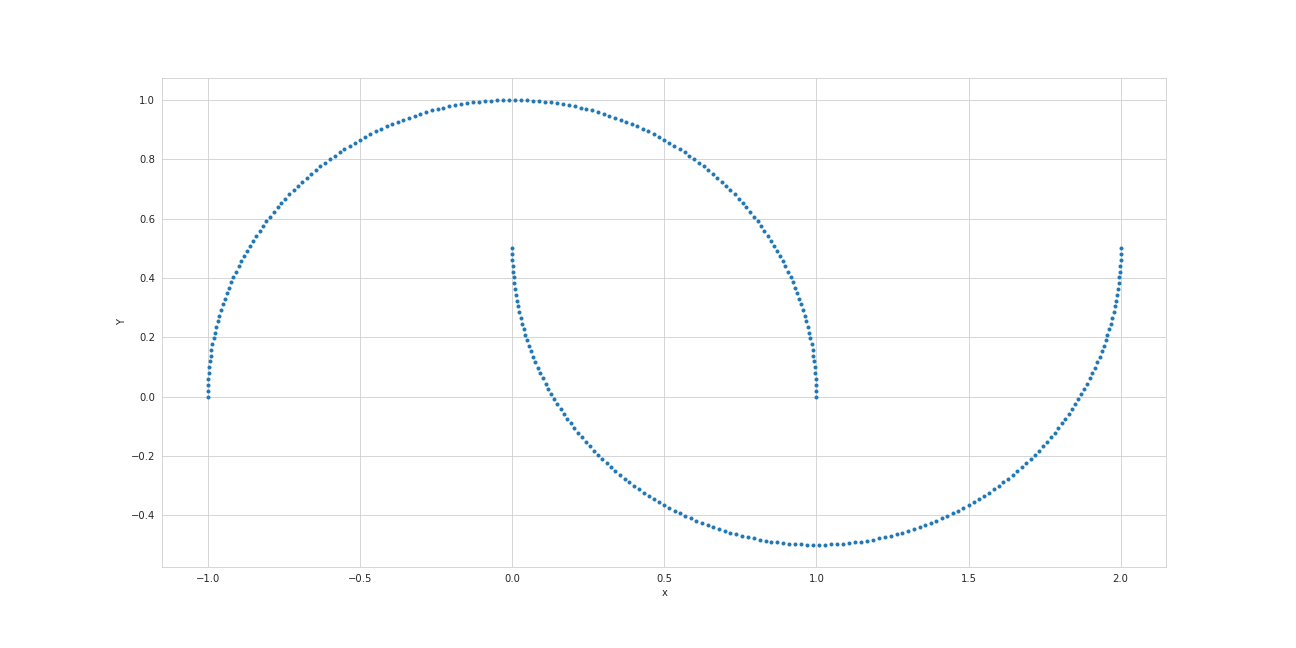
\includegraphics[width=0.95\textwidth, keepaspectratio]{images/make_moons_example.png}
    \caption{Here are represent an example of a set of 320 points of the toy dataset, i.e.
        two interleaving circles. These points are taken by setting noise to zero}
    \label{fig1}
\end{figure}
\newpage
\begin{figure}[!ht]
    \centering
    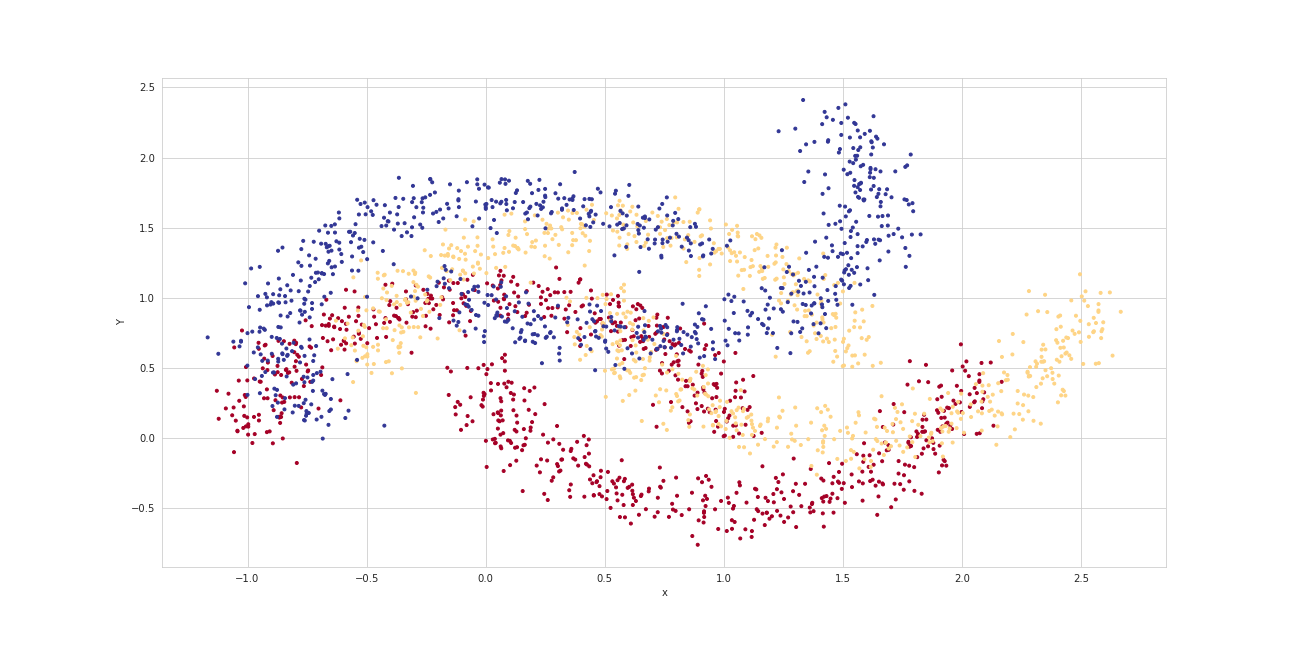
\includegraphics[width=0.95\textwidth, keepaspectratio]{images/datasets_examples.png}
    \caption{Here are shown three examples of the toy datasets. Are taken 840 points for 
        every dataset, with noise fixed at 0.1. The red dots represent the standard toy 
        dataset. The blue dots represent the rotated dataset by an angle of $\theta=\pi/5$.
        The yellow dots represent the traslated dataset using $dx=0.5$ and $dy=0.5$}
    \label{fig2}
\end{figure}
\begin{figure}[!hb]
    \centering
        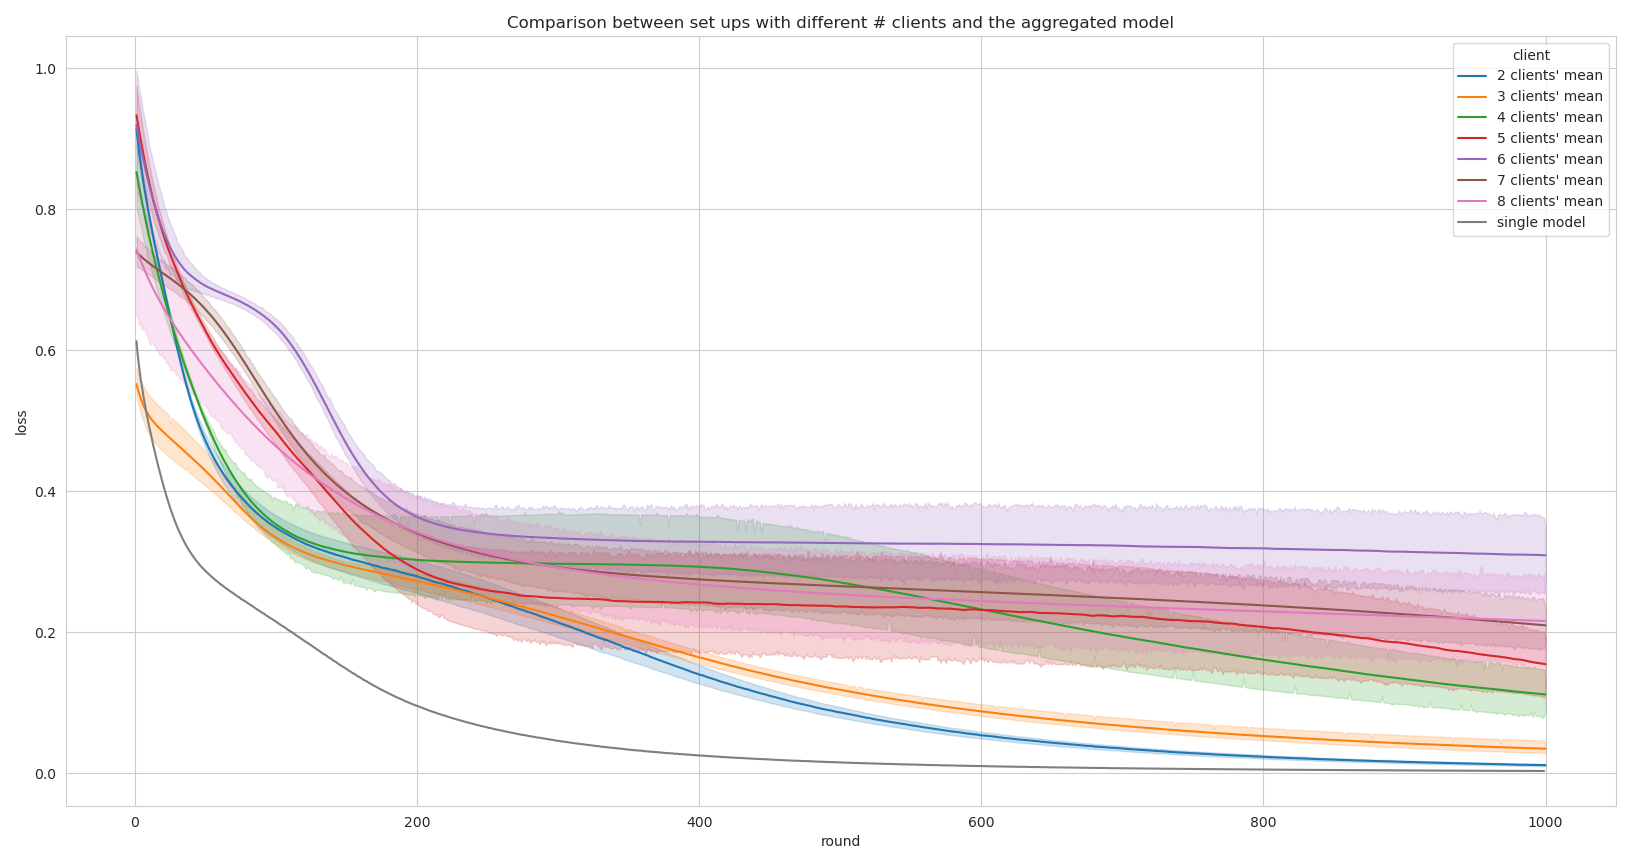
\includegraphics[width=0.95\textwidth, keepaspectratio]{images/loss_red_same.png}
    \caption{Here is represented the evolution of the loss function for different set ups, 
        summarized in the legend, in the number of epochs. For every curve, except for the 
        one referring to the aggregated model, is provided a confidence interval covering the 
        95\% of the true value.}
    \label{fig3}
\end{figure}
\newpage
\begin{figure}[!ht]
    \centering
        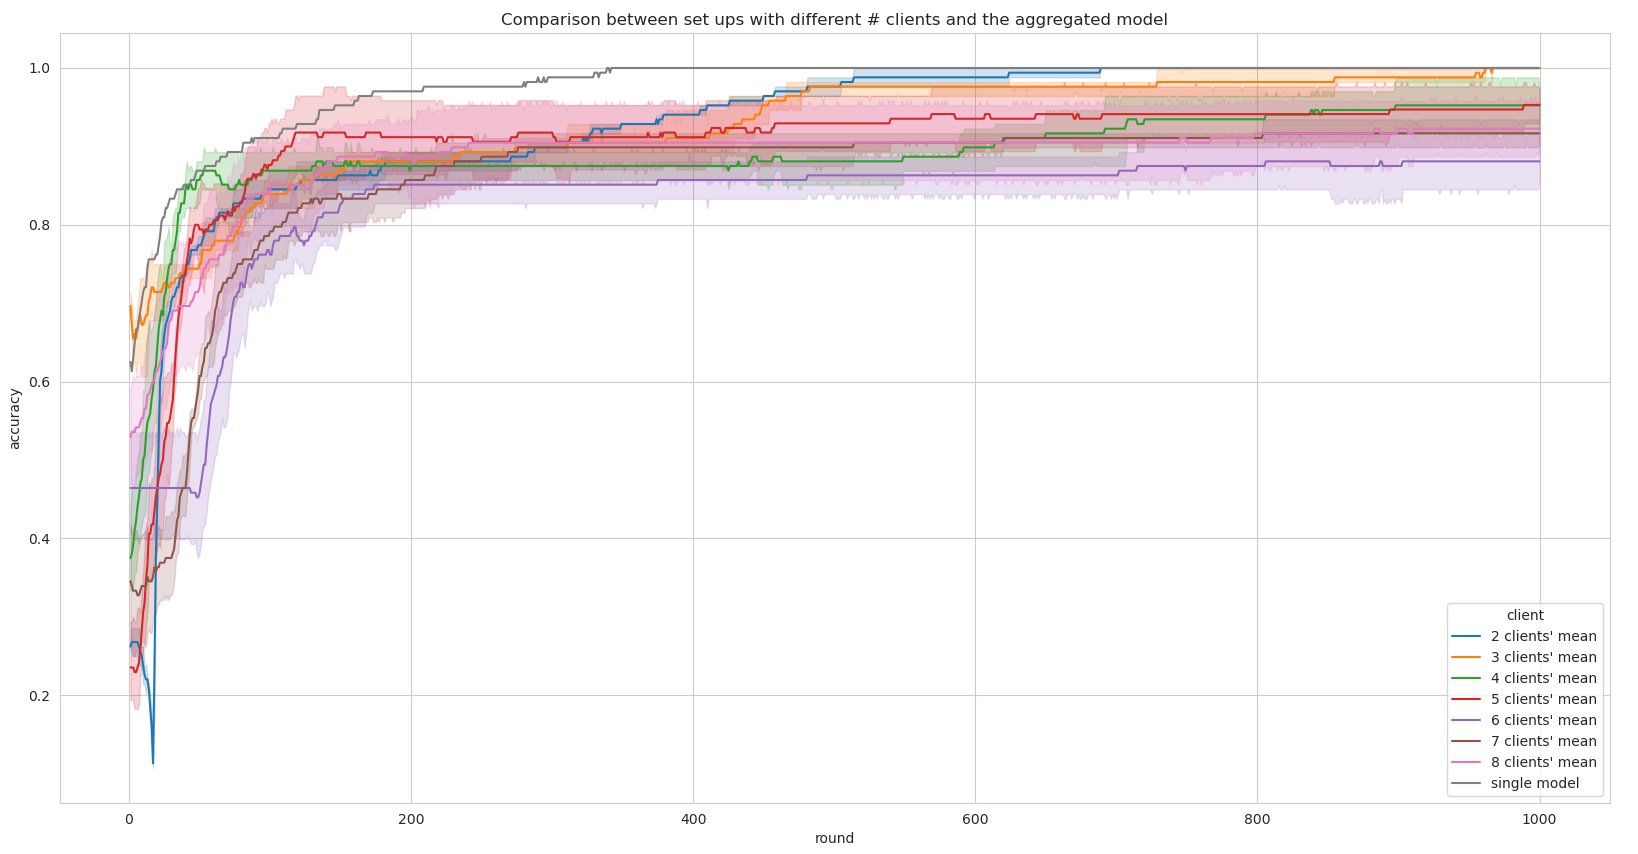
\includegraphics[width=0.95\textwidth, keepaspectratio]{images/accuracy_red_same.png}
    \caption{Here is represented the evolution of the accuracy function for different set ups, 
        summarized in the legend, in the number of epochs. For every curve, except for the 
        one referring to the aggregated model, is provided a confidence interval covering the 
        95\% of the true value.}
    \label{fig4}
\end{figure}
\begin{figure}[!hb]
    \centering
    \subfloat[]{
        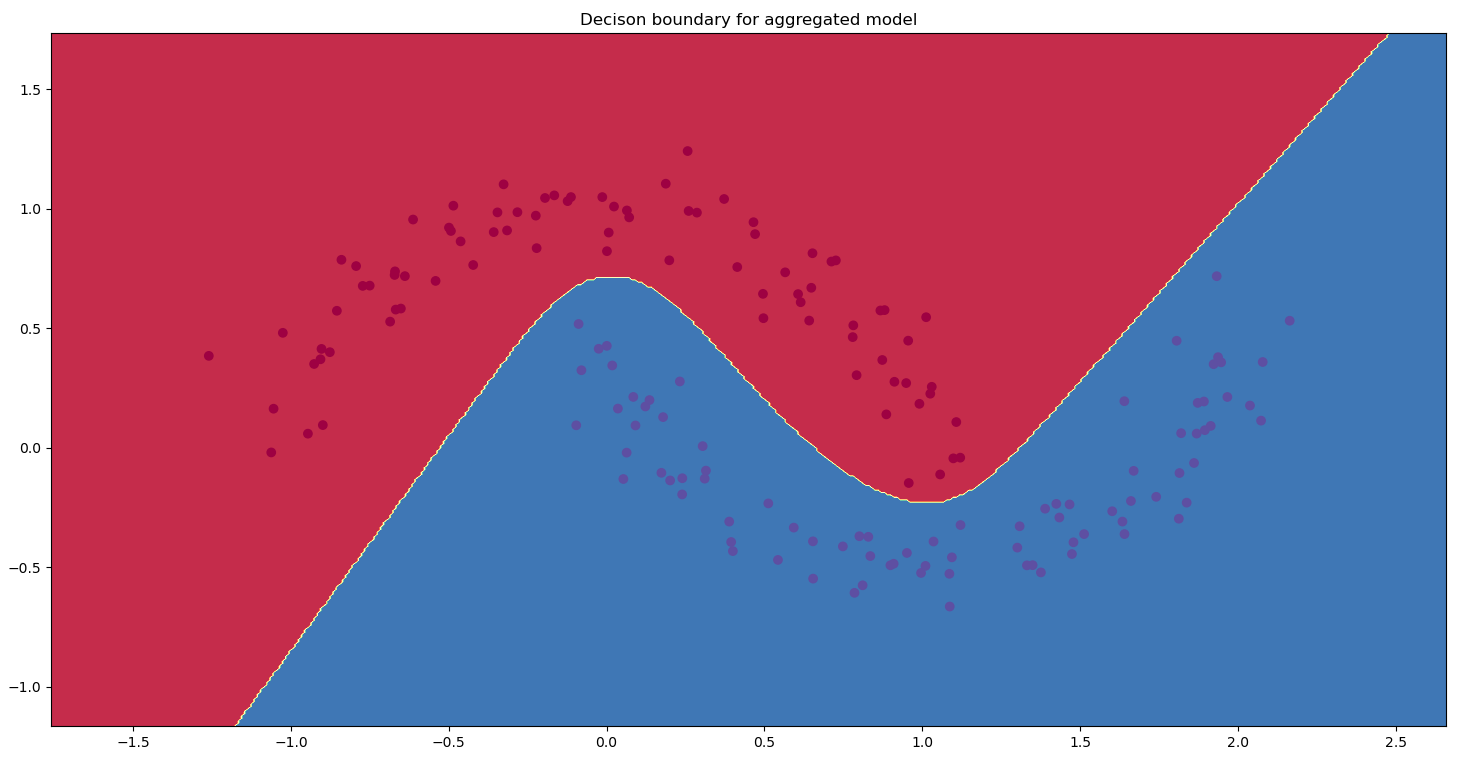
\includegraphics[width=0.45\textwidth, keepaspectratio]{images/db_single.png}
    }
    \subfloat[]{
        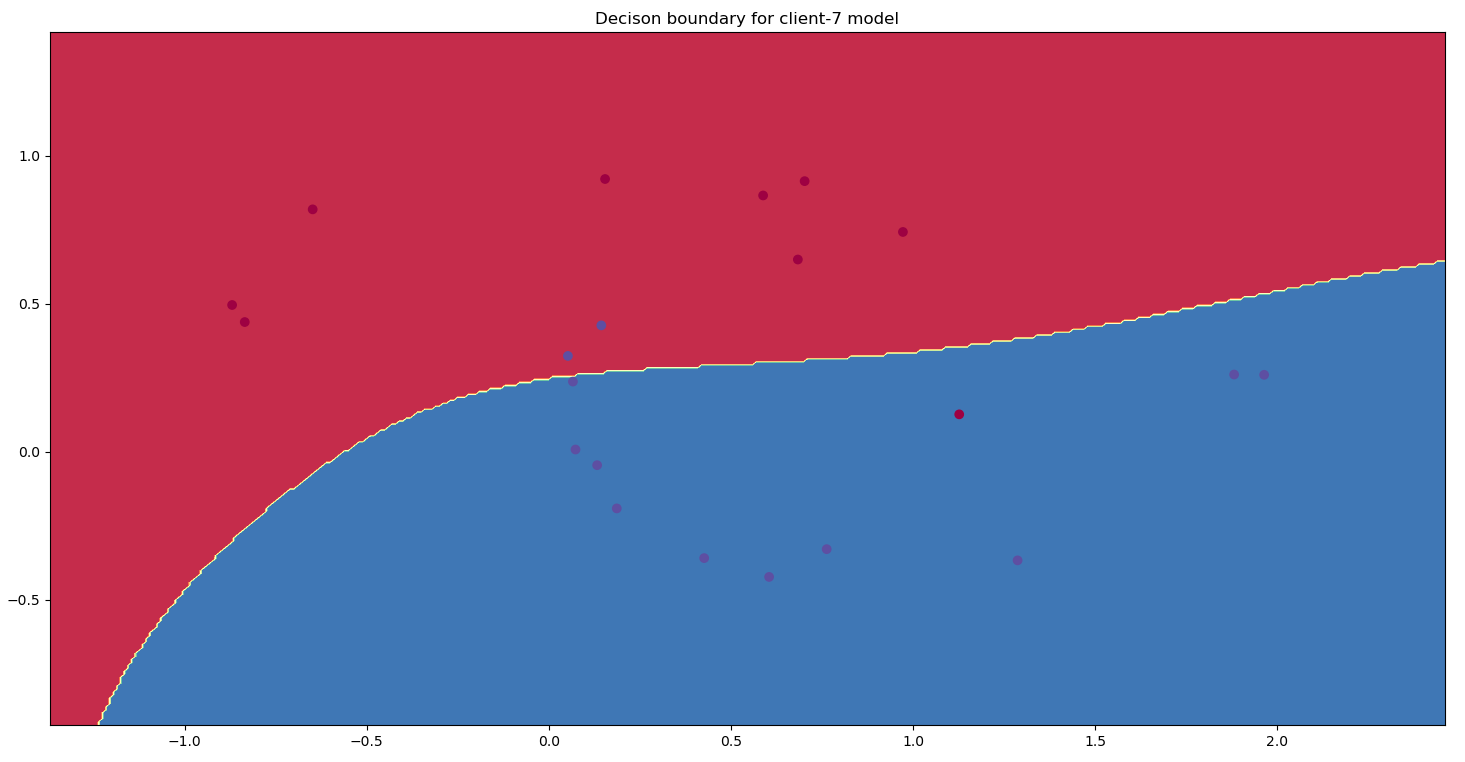
\includegraphics[width=0.45\textwidth, keepaspectratio]{images/db_distributed.png}
    }
    \caption{Here is provided a comparison between the final decision boundaries plotted on 
        the test dataset relative to (a) the aggregated model and (b) the $8-th$ client of 
        the FL set up.}
    \label{fig5}
\end{figure}
\newpage
\begin{figure}[!ht]
    \centering
        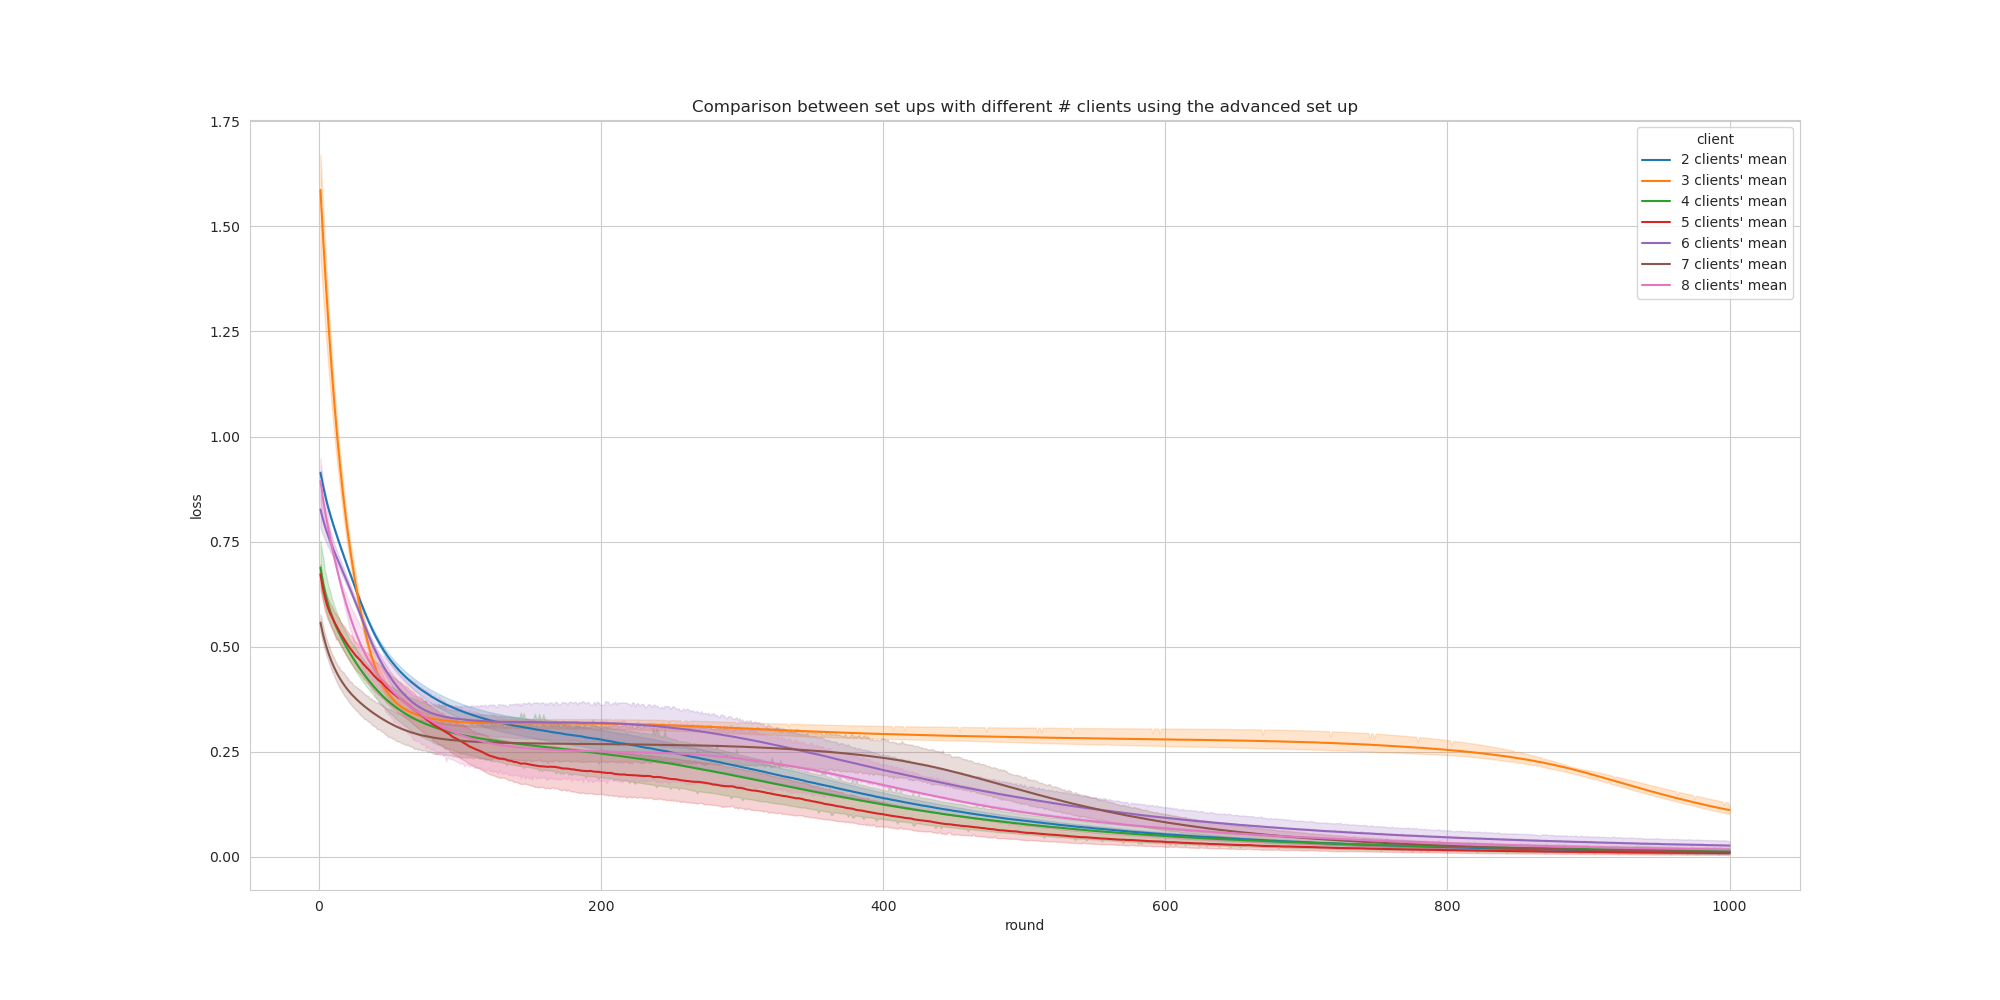
\includegraphics[width=0.95\textwidth, keepaspectratio]{images/loss_red_adv.png}
    \caption{Here is represented the evolution of the loss function for different set ups, 
        summarized in the legend, in the number of epochs. For every curve, is provided a confidence 
        interval covering the 95\% of the true value.}
    \label{fig6}
\end{figure}
\begin{figure}[!hb]
    \centering
        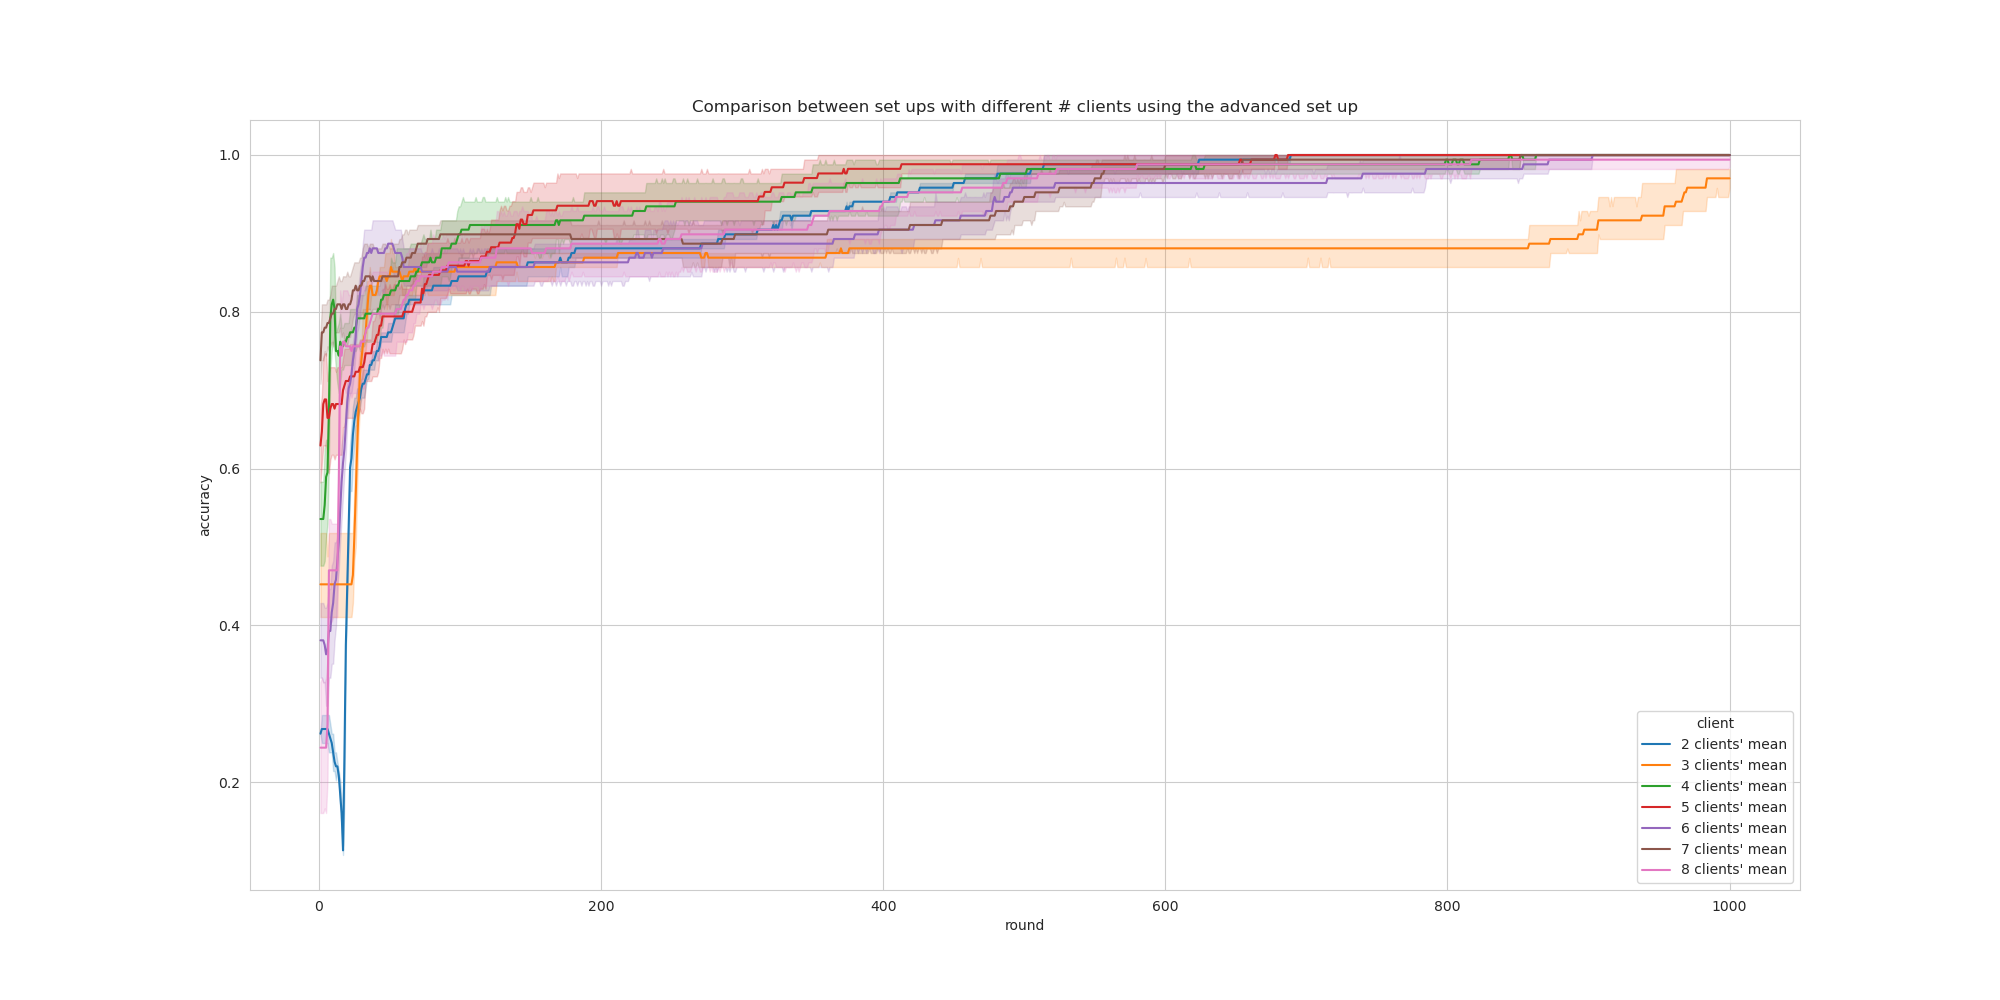
\includegraphics[width=0.95\textwidth, keepaspectratio]{images/accuracy_red_adv.png}
    \caption{Here is represented the evolution of the accuracy function for different set ups, 
        summarized in the legend, in the number of epochs. For every curve, is provided a confidence 
        interval covering the 95\% of the true value.}
    \label{fig7}
\end{figure}
\newpage
\begin{figure}[!ht]
    \centering
        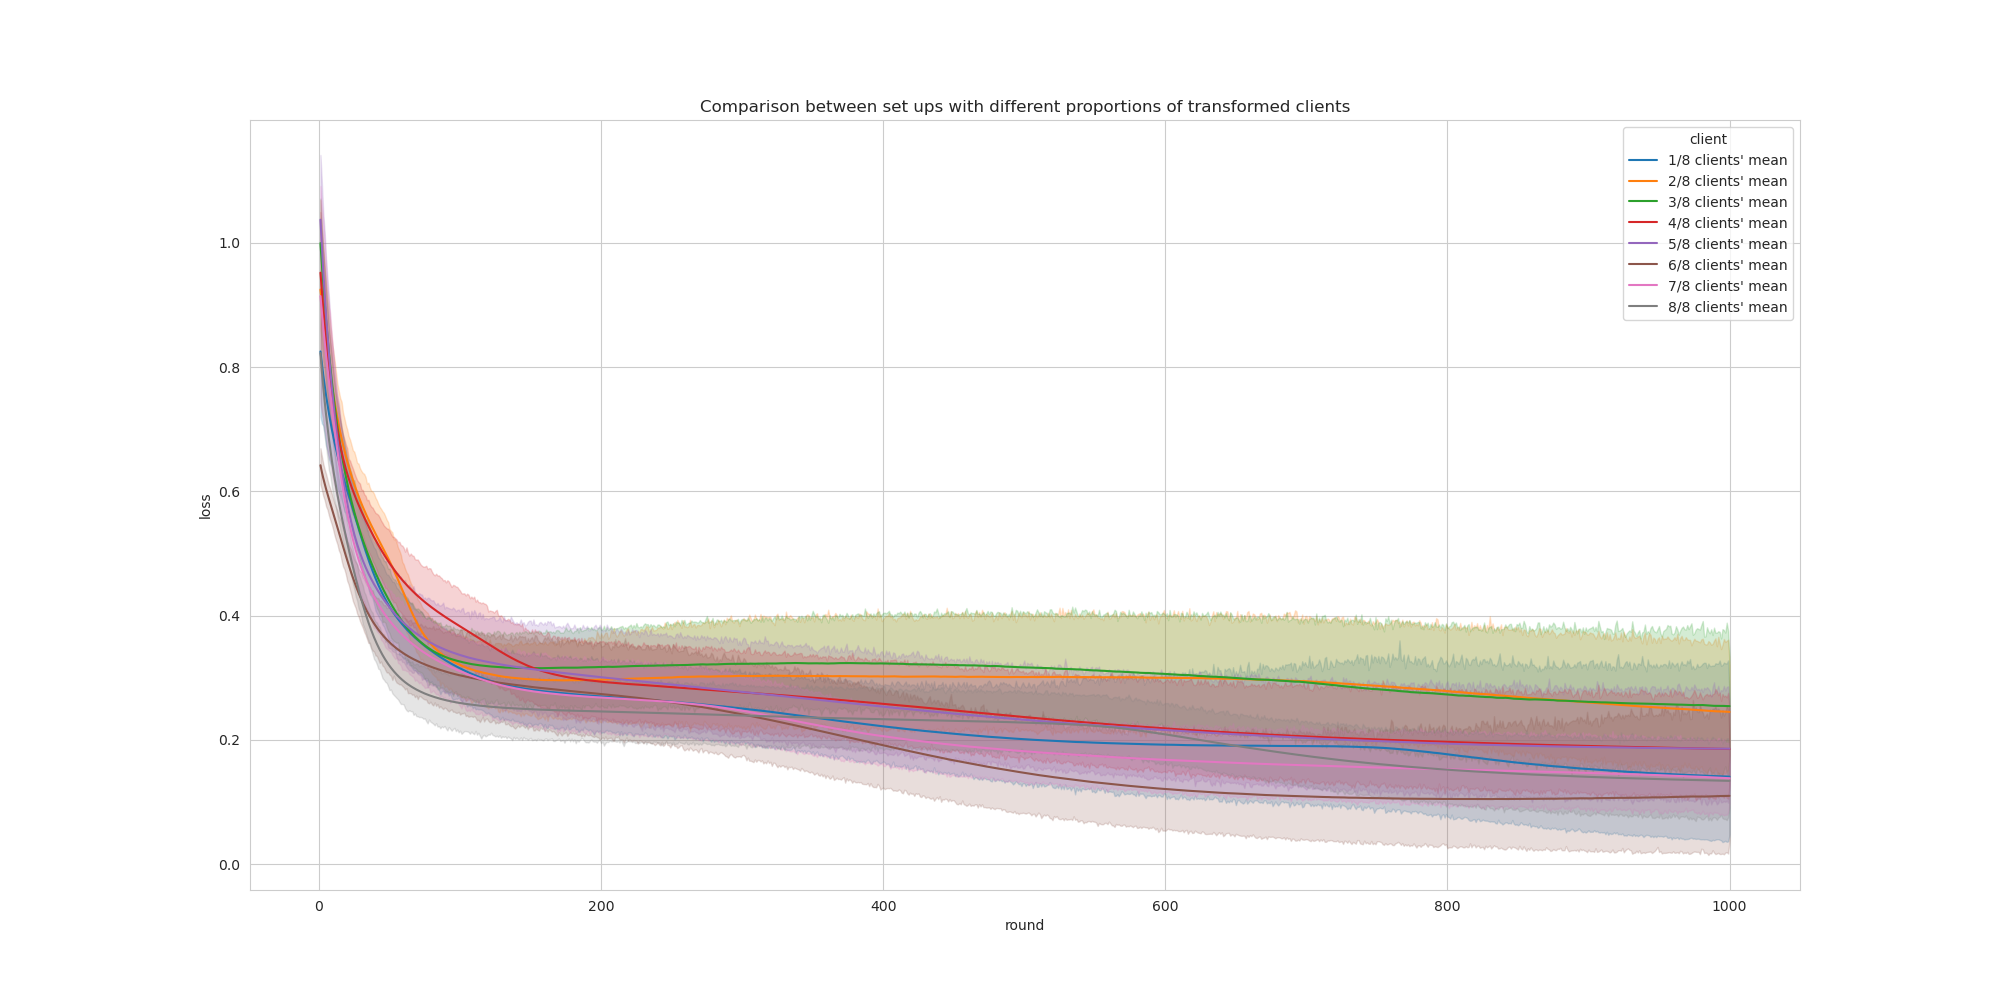
\includegraphics[width=0.95\textwidth, keepaspectratio]{images/loss_red_TL2.png}
    \caption{Here is represented the evolution of the loss function for different set ups, 
    summarized in the legend, in the number of epochs. For every curve, is provided a confidence 
    interval covering the 95\% of the true value. The fractions that define the set ups in the 
    legend refer to the fraction of clients in tht set up having a rotated dataset.}
    \label{fig8}
\end{figure}
\begin{figure}[!hb]
    \centering
        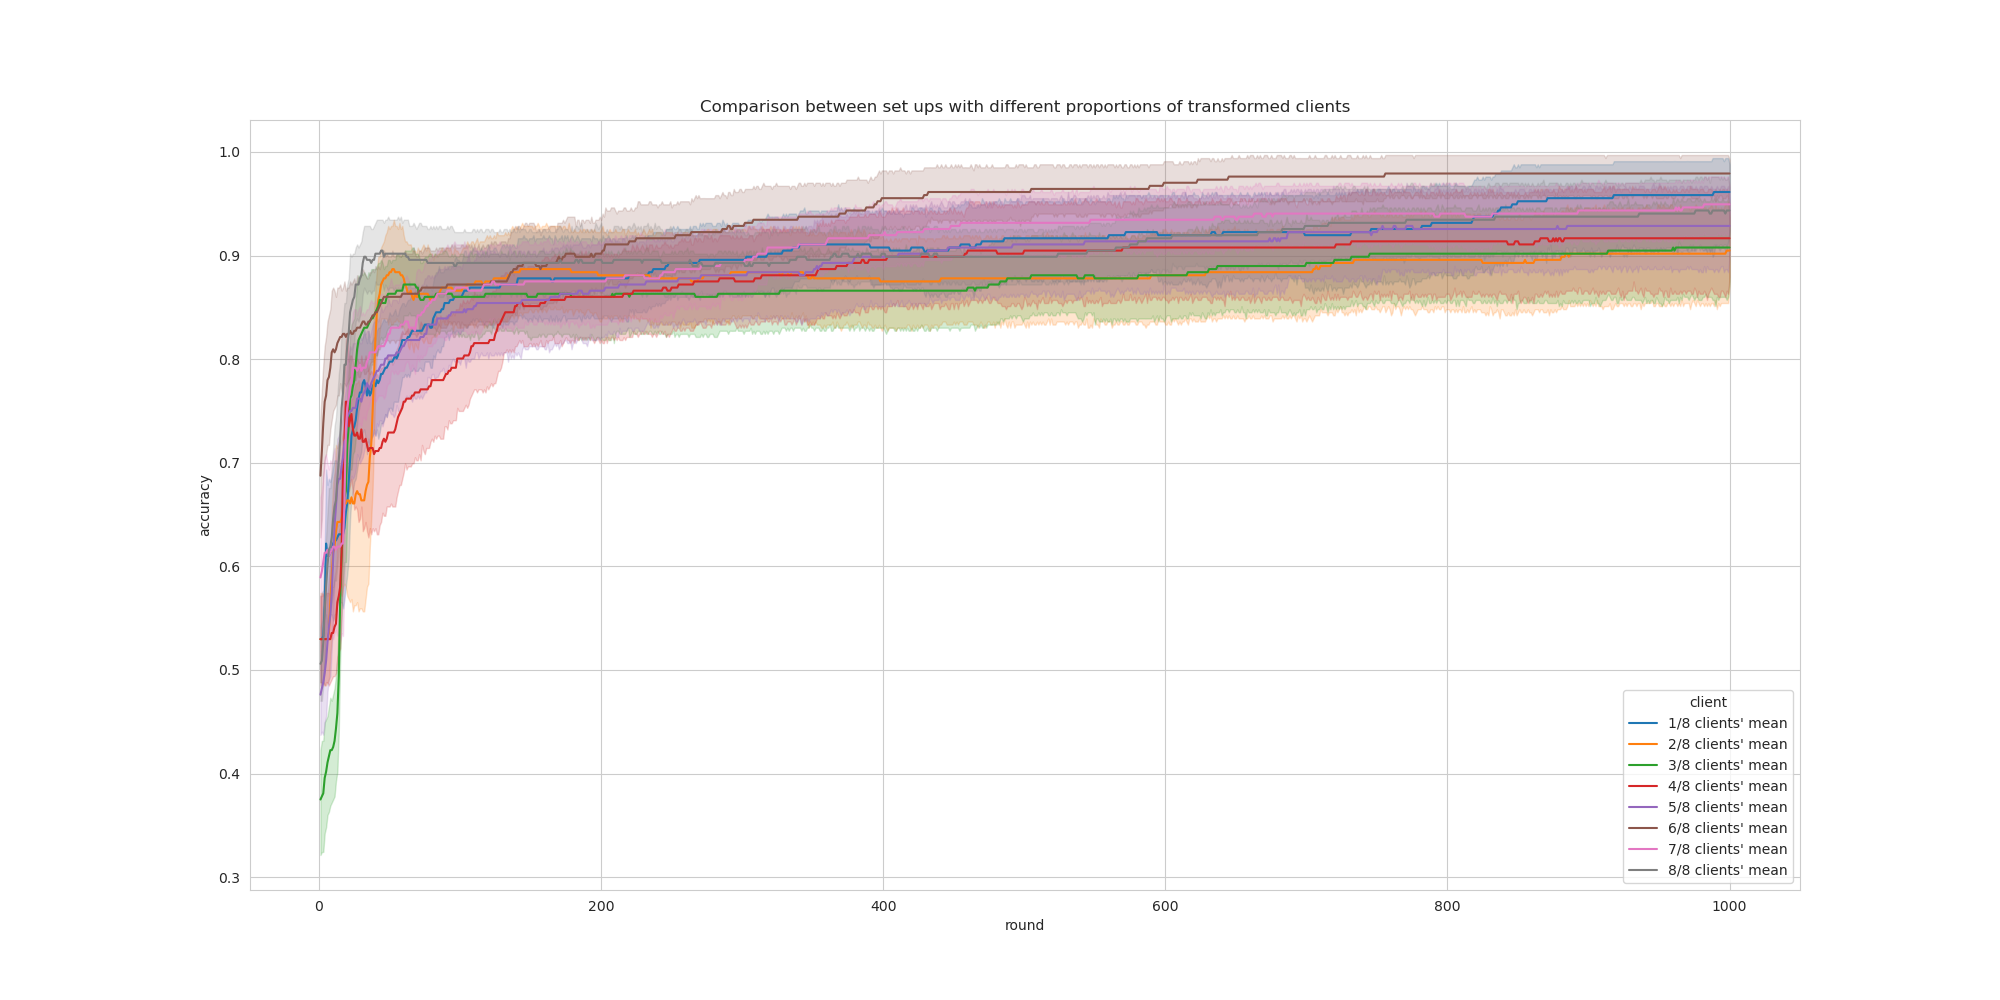
\includegraphics[width=0.95\textwidth, keepaspectratio]{images/accuracy_red_TL2.png}
    \caption{Here is represented the evolution of the accuracy function for different set ups, 
    summarized in the legend, in the number of epochs. For every curve, is provided a confidence 
    interval covering the 95\% of the true value. The fractions that define the set ups in the 
    legend refer to the fraction of clients in tht set up having a rotated dataset.}
    \label{fig9}
\end{figure}
\newpage
\begin{figure}[!ht]
    \centering
        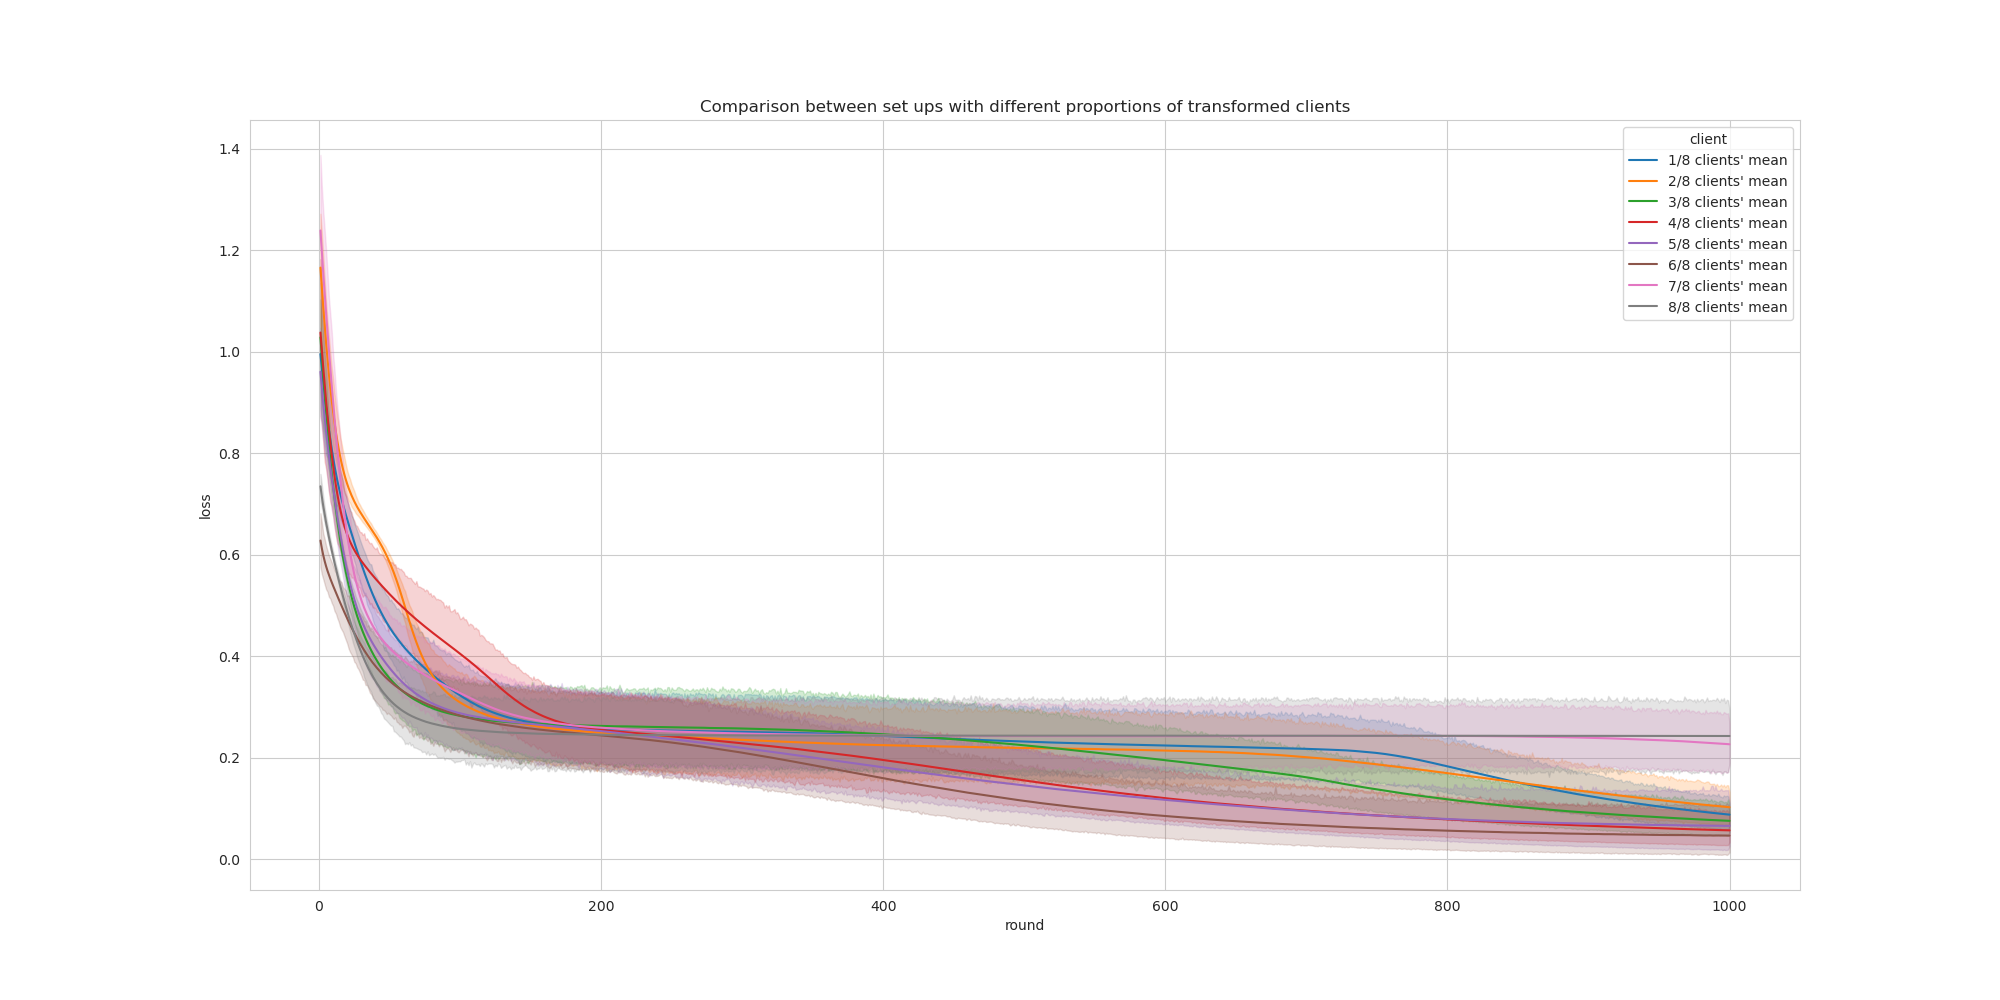
\includegraphics[width=0.95\textwidth, keepaspectratio]{images/loss_red_TL1.png}    
    \caption{Here is represented the evolution of the loss function for different set ups, 
    summarized in the legend, in the number of epochs. For every curve, is provided a confidence 
    interval covering the 95\% of the true value. The fractions that define the set ups in the 
    legend refer to the fraction of clients in tht set up having a traslated dataset.}
    \label{fig10}
\end{figure}
\begin{figure}[!hb]
    \centering
        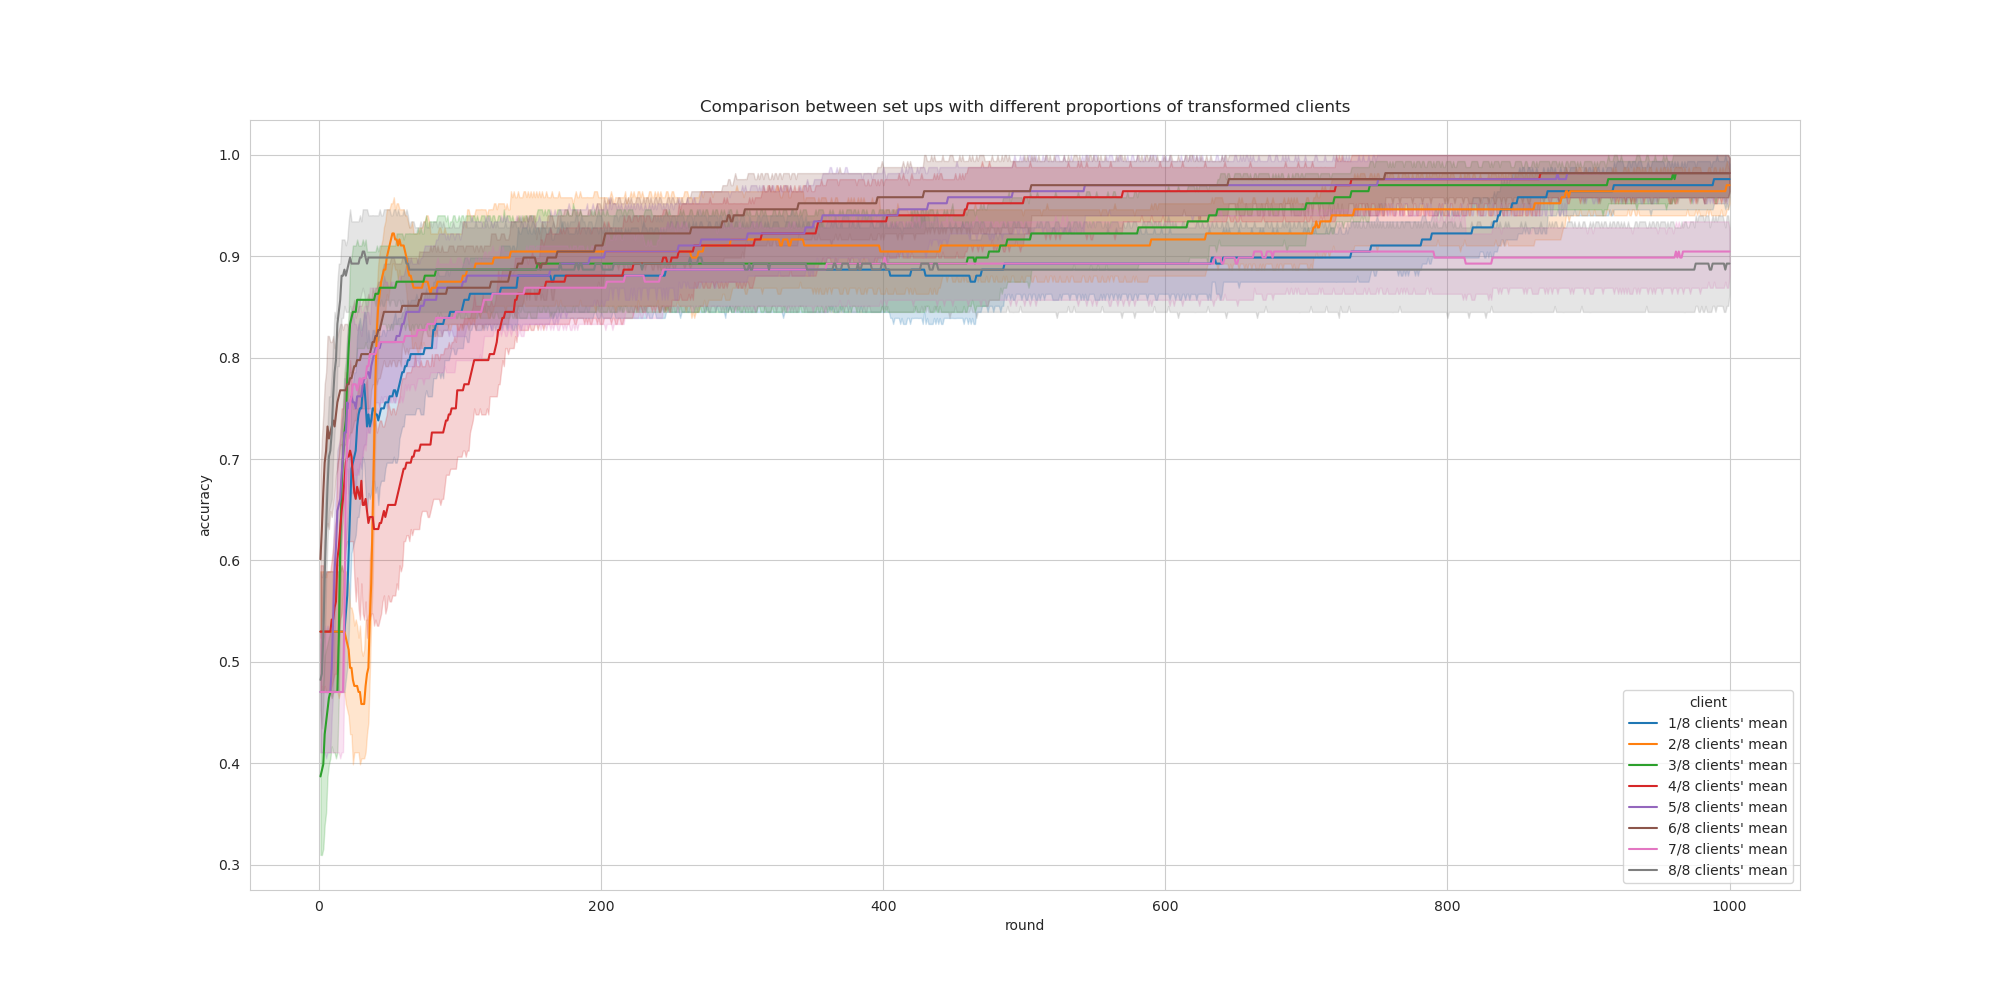
\includegraphics[width=0.95\textwidth, keepaspectratio]{images/accuracy_red_TL1.png}
    \caption{Here is represented the evolution of the accuracy function for different set ups, 
    summarized in the legend, in the number of epochs. For every curve, is provided a confidence 
    interval covering the 95\% of the true value. The fractions that define the set ups in the 
    legend refer to the fraction of clients in tht set up having a traslated dataset.}
    \label{fig11}
\end{figure}



%###############################################


\newpage
\bibliographystyle{unsrt}
\bibliography{bibliography}

\renewcommand\thefigure{\thesection.\arabic{figure}}
\end{document} % NOTHING AFTER THIS LINE IS PART OF THE DOCUMENT